\section{Experimental Setup}
\subsection{Research Questions}

We evaluate the performance of SOTA LLM-based agents on realistic feature-level code generation with FeatBench. Specifically, we aim to address the following research questions (RQs):
\begin{itemize}
    \item RQ1: How do different agent frameworks compare in their performance to implement features from realistic natural language requirements?
    \item RQ2: Which factors influence the resolved rate of different agents, and which do not?
    \item RQ3: What are the primary failure reasons for agents on FeatBench, and how do their behavioral patterns influence the quality and reliability of feature implementations?
\end{itemize}

\subsection{Model Selection}
Completing a realistic feature implementation task in FeatBench typically requires a deep understanding of the target repository, demanding strong reasoning ability and the capacity to handle very long contexts. To meet these rigorous demands and evaluate the upper bounds of current capabilities, we selected four SOTA LLMs as backbones, encompassing both proprietary and open-source models:
the open-source DeepSeek V3.1 (deepseek-chat), and three proprietary models: GPT-5 (gpt-5-2025-08-07), Doubao-Seed-1.6 (doubao-seed-1-6-250615), and Qwen3-Coder-Flash (qwen3-coder-flash-2025-07-28).
To ensure reproducibility and minimize randomness in generation, all LLMs are configured with a temperature of $0.0$ and a top-p value of $1.0$.

\subsection{Agent Frameworks}
Due to the complexity of realistic feature implementation tasks, directly prompting LLMs to generate the required changes is infeasible. Therefore, to investigate RQ1, we selected two representative agent frameworks.
Agentless~\cite{agentless} is a pipeline-based agent, employing a rigid, two-stage pipeline consisting of feature localization and patch generation. It emphasizes cost-effectiveness and stability but lacks the flexibility to handle implicit cross-file dependencies. Following the methodology in SWE-bench-Live~\cite{swebenchgoeslive}, we generally adhered to the original pipeline settings but omitted the regression testing-based reranking stage because supporting this stage requires substantial infrastructure adaptation beyond our scope. Consequently, our evaluation of Agentless produces a single candidate solution per task. In contrast, Trae-agent~\cite{traeagent} is an autonomous planning agent, utilizing a ReAct loop~\cite{yao2022react} to dynamically plan execution paths and utilize tools. This design allows for iterative reasoning and stronger environment exploration capabilities. For our experiments, we imposed a maximum limit of 150 steps per task and equipped the agent with supplementary tools, including \texttt{ckg} (code knowledge graph) and \texttt{json\_edit\_tool}.

\subsection{Evaluation Metrics}
Following the standards set by previous works~\cite{swebench, deng2025nocode}, we adopt the \textbf{Resolved Rate (\%)} as our primary metric.
This measures the percentage of feature implementation tasks an agent successfully completes. 
We also report the \textbf{Patch Apply Rate (\%)}, which indicates the proportion of generated patches that are syntactically correct and can be applied to the repository without errors.
Furthermore, we measure the \textbf{File-level Localization Success Rate (\%)}, which assesses whether the set of files modified by the generated patch matches the ground-truth patches.
In addition, we introduce three auxiliary metrics to facilitate a more in-depth analysis of test case outcomes:
\begin{itemize}
    \item \textbf{Feature Validation Pass Rate (\%):} This metric evaluates the correctness and completeness of the feature implementation by measuring the pass rate of the F2P test cases.
    \item \textbf{Regression Tests Pass Rate (\%):} Critical for ensuring system stability, this metric measures the proportion of tasks that maintain system reliability, evaluated by the pass rate of the P2P test cases.
    \item \textbf{Tokens Cost:} The average number of tokens consumed per task, reflecting the economic efficiency.
\end{itemize}

\section{Results}
\subsection{RQ1: Performance Evaluation on FeatBench}
\begin{table}[t!]
    \centering
    \caption{Performance comparison across different agents \& LLMs on
    FeatBench. }
    \begin{adjustbox}
        {width=\textwidth}
        \setlength{\tabcolsep}{3pt}
        \begin{tabular}{ccccccc|cccccc}
            \toprule \multirow{2}{*}{\textbf{Model}}                                 & \multicolumn{6}{c}{\textbf{Trae-agent}} & \multicolumn{6}{c}{\textbf{Agentless}} \\
            \cmidrule{2-13}                                                          & \textbf{Resolved\%}                     & \textbf{Applied\%}                    & \textbf{RT\%}    & \textbf{FV\%}    & \textbf{File\%}  & \textbf{\#Token} & \textbf{Resolved\%} & \textbf{Applied\%} & \textbf{RT\%}    & \textbf{FV\%}    & \textbf{File\%}  & \textbf{\#Token} \\
            \midrule \multicolumn{13}{c}{\cellcolor{lb} \textbf{Open-Source Model}}   \\
            \textbf{DeepSeek V3.1}                                                   & 22.29\%                                 & \textbf{100.00\%}                     & 42.68\%          & 46.50\%          & 79.11\%          & 2.21M            & 9.55\%              & 70.70\%            & 32.48\%          & 19.11\%          & 42.28\%          & 0.05M            \\
            \midrule \multicolumn{13}{c}{\cellcolor{lb} \textbf{Closed-Source Model}} \\
            \midrule \textbf{Doubao-Seed-1.6}                                        & 15.92\%                                 & \textbf{100.00\%}                     & 41.40\%          & 26.75\%          & 65.77\%          & 1.07M            & 10.19\%             & 91.72\%            & 26.75\%          & 19.11\%          & 49.30\%          & 0.08M            \\
            \textbf{Qwen3-Coder-Flash}                                               & 20.38\%                                 & \textbf{100.00\%}                     & \textbf{50.32\%} & 37.58\%          & 74.37\%          & 1.72M            & 7.00\%              & 71.34\%            & 24.84\%          & 14.01\%          & 36.49\%          & 0.05M            \\
            \textbf{GPT-5}                                                           & \textbf{29.94\%}                        & \textbf{100.00\%}                     & \textbf{50.32\%} & \textbf{56.05\%} & \textbf{86.43\%} & 2.90M            & \textbf{16.56\%}    & \textbf{98.09\%}   & \textbf{35.67\%} & \textbf{34.39\%} & \textbf{67.54\%} & 0.07M            \\
            \midrule\midrule \textbf{Average}                                        & 22.13\%                                 & 100.00\%                              & 46.18\%          & 41.72\%          & 76.42\%          & 1.98M            & 10.83\%             & 82.96\%            & 29.94\%          & 21.66\%          & 48.90\%          & 0.06M            \\
            \bottomrule
        \end{tabular}
    \end{adjustbox}
    \label{tab:performance}
\end{table}

\begin{wrapfigure}{r}{0.45\textwidth}
    \vspace{-45pt}
    \centering
    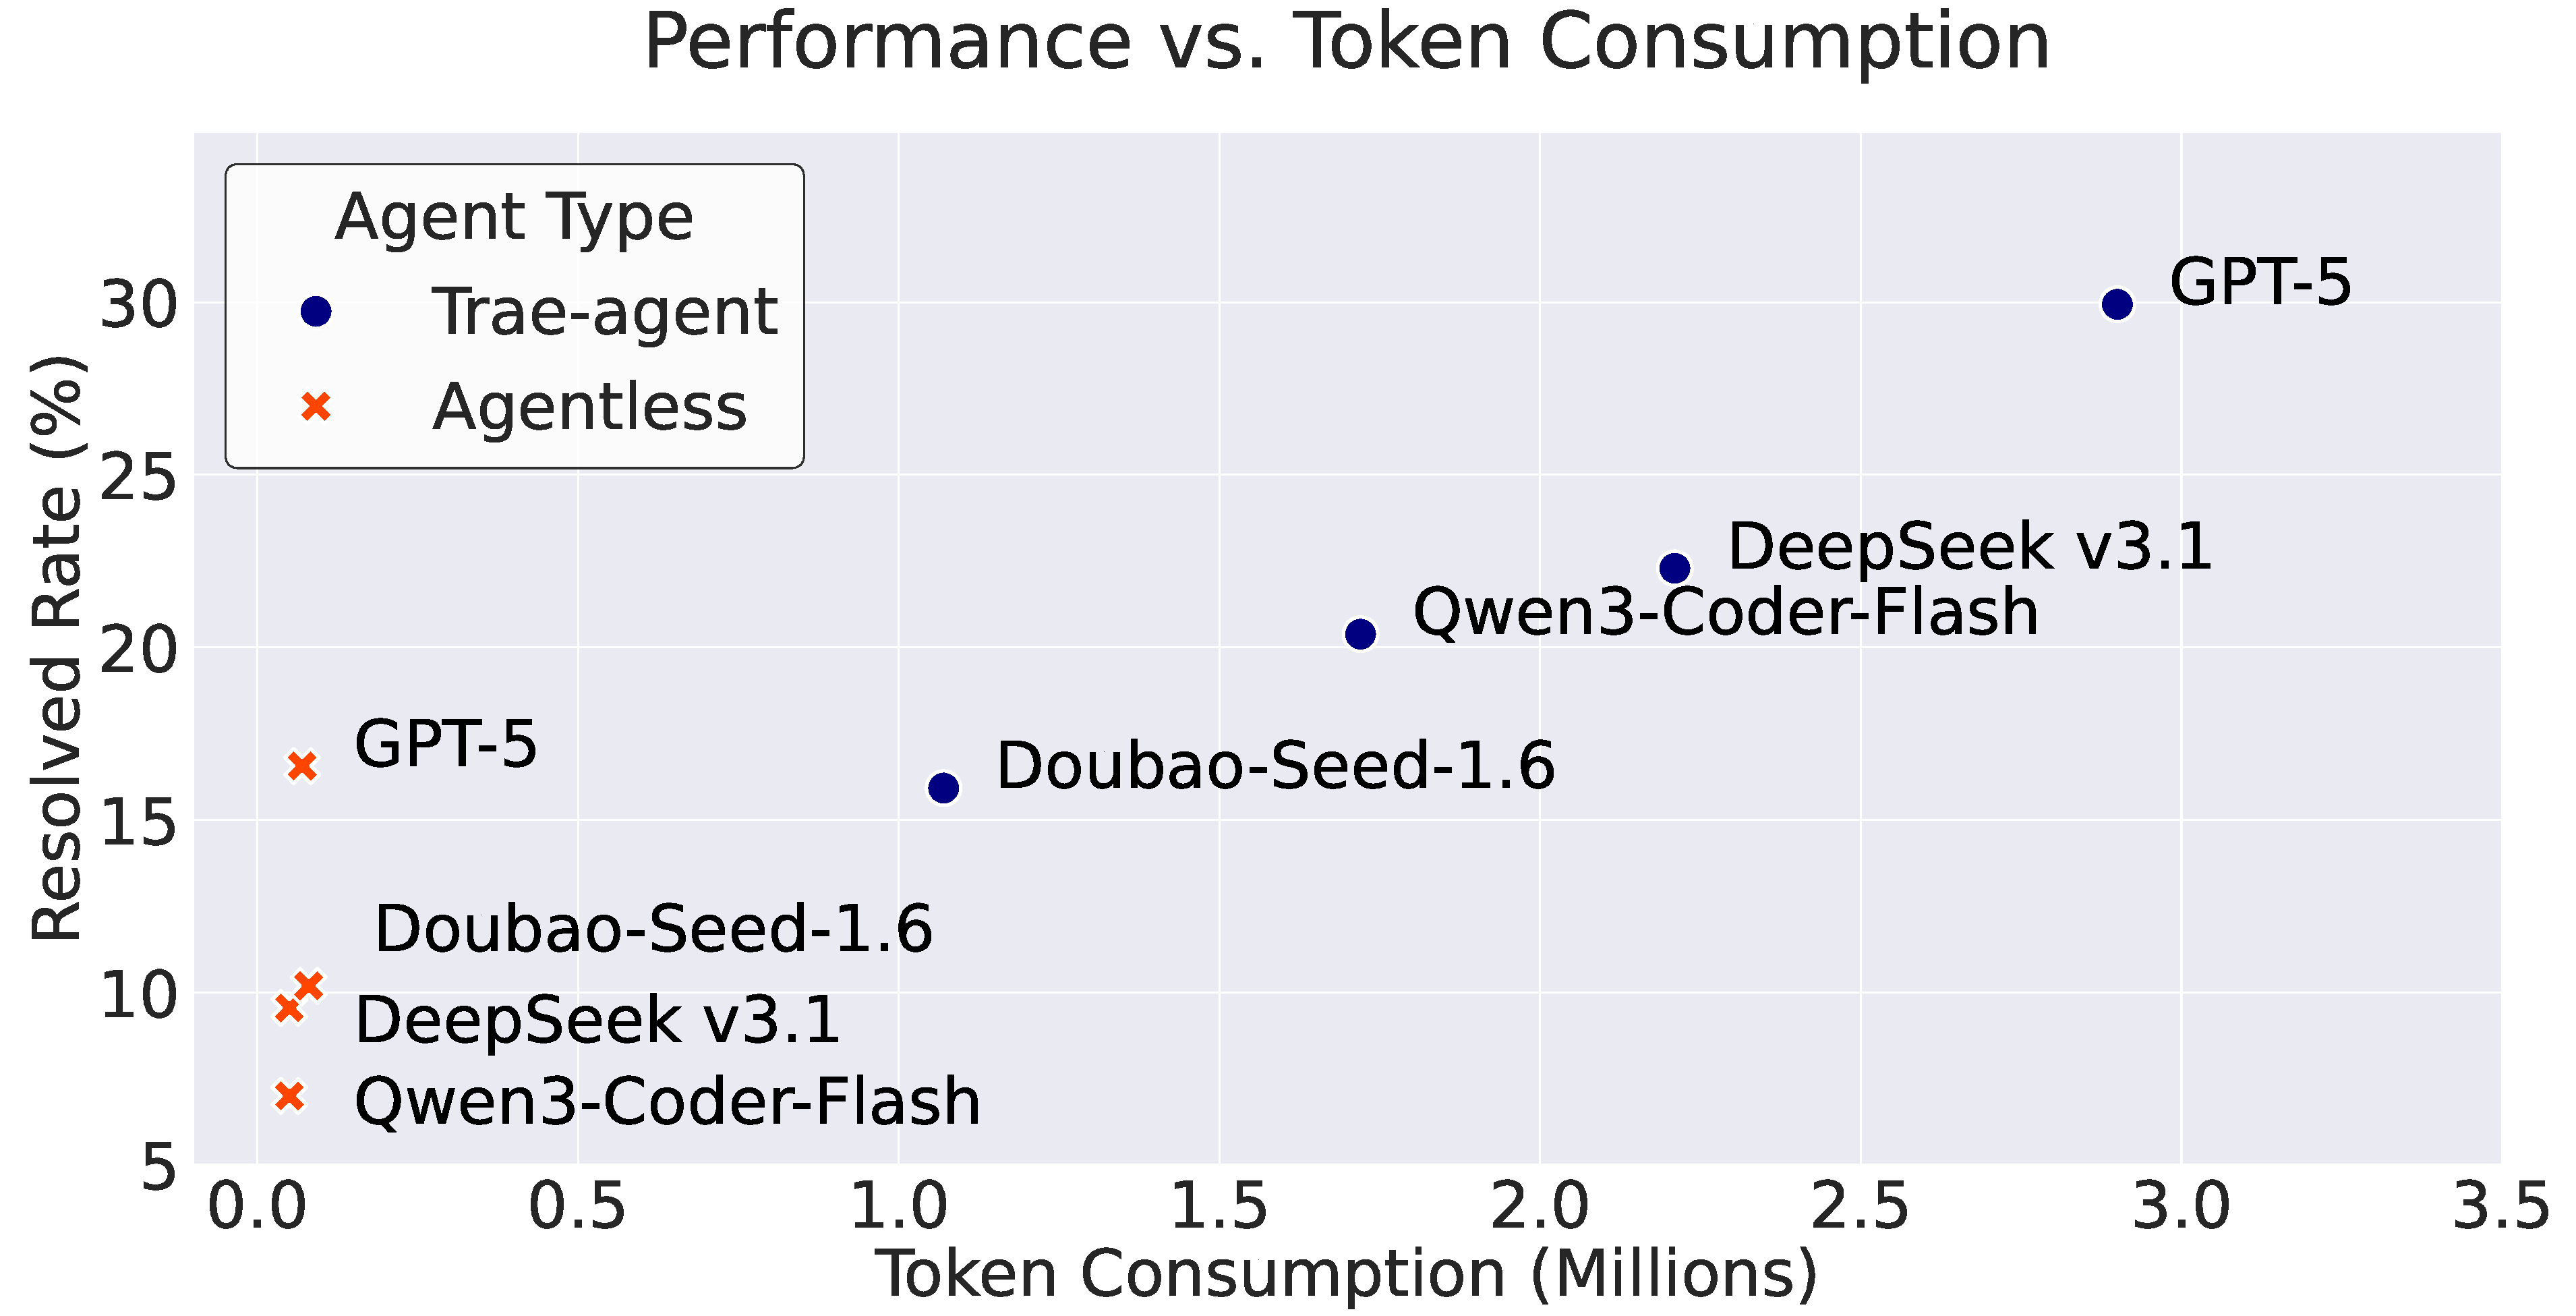
\includegraphics[width=\linewidth]{figs/Figure_6.pdf}
    \caption{Association between Token Consumption and Resolved Rate.}
    \Description{A scatter plot illustrating the trade-off between computational cost and performance.}
    \label{fig:token}
    \vspace{-15pt}
\end{wrapfigure}

The performance results of all agent-model configurations on FeatBench are reported in \cref{tab:performance}.
Overall, the evaluation highlights the challenging nature of FeatBench, which poses a significant hurdle for the SOTA configuration. 
\textbf{Even equipped with the advanced GPT-5 model, the autonomous Trae-agent achieves a Resolved\% of only 29.94\%.} 
This low performance ceiling underscores the inherent difficulty of realistic feature implementation tasks.

Alongside the overall task difficulty, our evaluation further reveals a clear divergence in performance between different agent frameworks.
\textbf{Autonomous frameworks demonstrate superior capability compared to pipeline-based ones in handling complex development scenarios.}
Trae-agent consistently outperforms Agentless across key metrics, driven by its ability to autonomously plan execution paths and utilize external tools.
A significant gap is evident in the functional correctness of the generated patches: Trae-agent achieves average Feature Validation (FV\%) and Regression Testing (RT\%) scores of 41.72\% and 46.18\% respectively, whereas Agentless performs substantially worse, with its average FV\% and RT\% dropping to 21.66\% and 29.94\%.
This disparity extends to localization capabilities. Trae-agent's average File\% of 76.42\% far surpasses Agentless's 48.90\%, indicating that dynamic planning is essential for accurately identifying modification targets in large repositories.
However, these performance gains come at the cost of significantly higher token consumption. As illustrated in \cref{fig:token}, Trae-agent exhibits a near-linear trend where achieving a higher resolved rate requires proportionally greater token consumption, ranging from 1.07M to 2.90M. In contrast, while the rigid process of Agentless is highly token-efficient, consistently operating under 0.1M tokens, its Resolved\% remains limited to a lower range of 7.00\% to 16.56\%.

Despite the performance differences between frameworks, a universal challenge persists across all model combinations regarding reliability. 
\textbf{We observe a universally low Regression Tests Pass Rate (RT\%), revealing a significant risk of agents introducing regressions while implementing new features.} 
This high risk of regression directly undermines the reliability required for production environments, where maintaining system stability remains a non-negotiable requirement.

\begin{boxK}
\textbf{RQ1 Summary:} 
Our evaluation reveals that FeatBench presents a significant challenge, with even SOTA configurations achieving a maximum Resolved\% of only 29.94\%. While autonomous planning agents significantly outperform rigid pipeline-based ones, their superior performance is currently inextricably linked to higher token consumption. Crucially, all evaluated agents exhibit a propensity for introducing software regressions, highlighting a critical reliability bottleneck for deploying agents in production environments.
\end{boxK}

\begin{figure}[t]
    \centering
    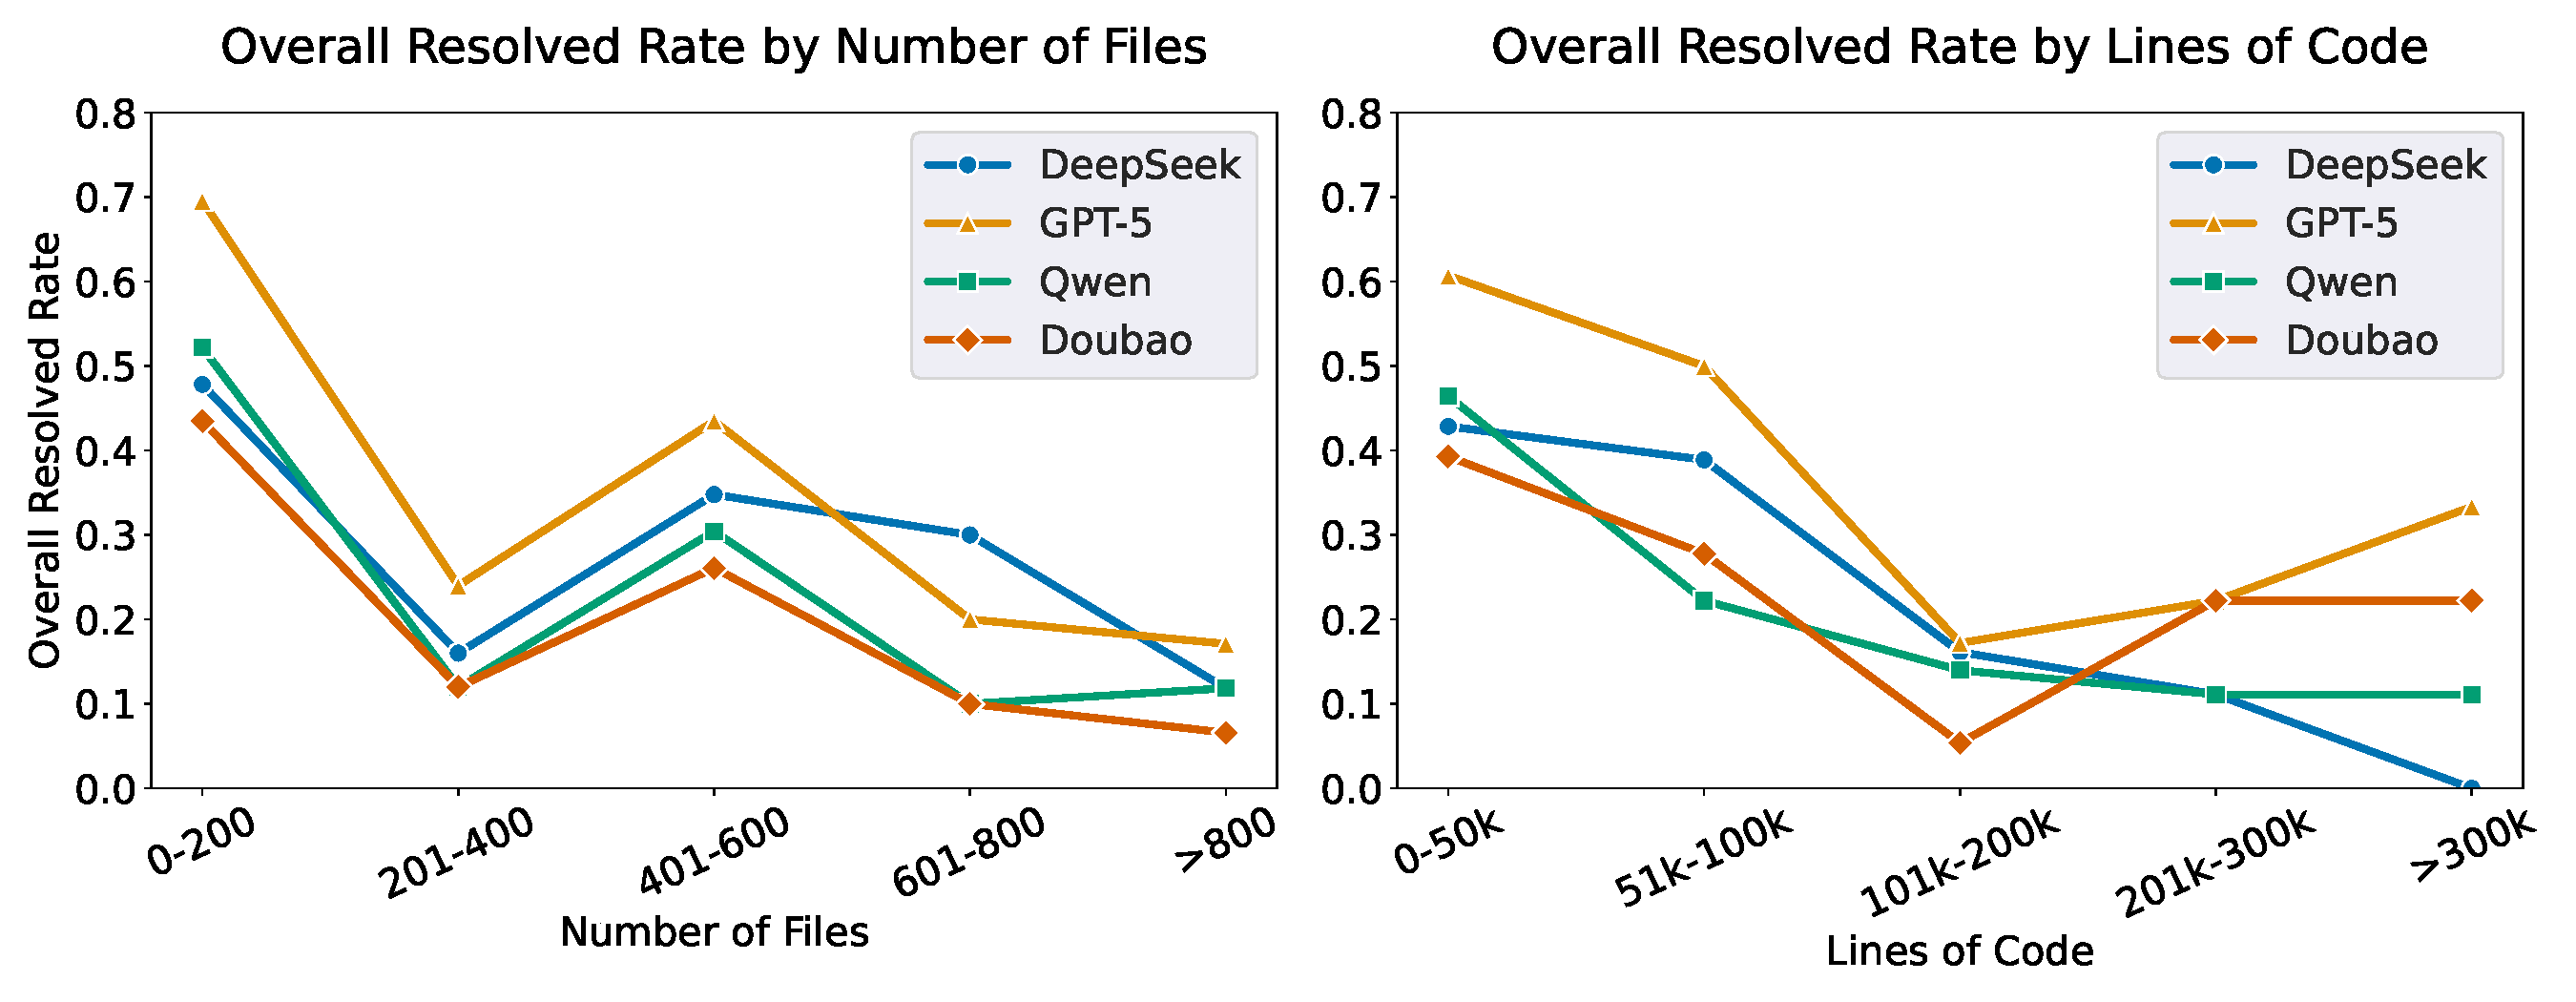
\includegraphics[width=\linewidth]{figs/Figure_1.pdf}
    \caption{Resolved Rate in Relation to Repository Complexity.}
    \Description{A dual-pane visualization showing the correlation between repository complexity and agent performance. The left plot measures complexity by the total number of files, while the right plot uses the aggregate Lines of Code (LoC). Both plots display a clear inverse relationship, where the Resolved Rate of agents significantly decreases as the repository scale increases.}
    \label{fig:repository_complexity}
\end{figure}
\subsection{RQ2: Factors Influencing Resolved Rate}
To answer RQ2, we investigate the influence of two potential factors on agent performance: task complexity at both the repository and patch levels, and task creation time.

\begin{wrapfigure}{r}{0.45\textwidth}
    \vspace{-32pt}
    \centering
    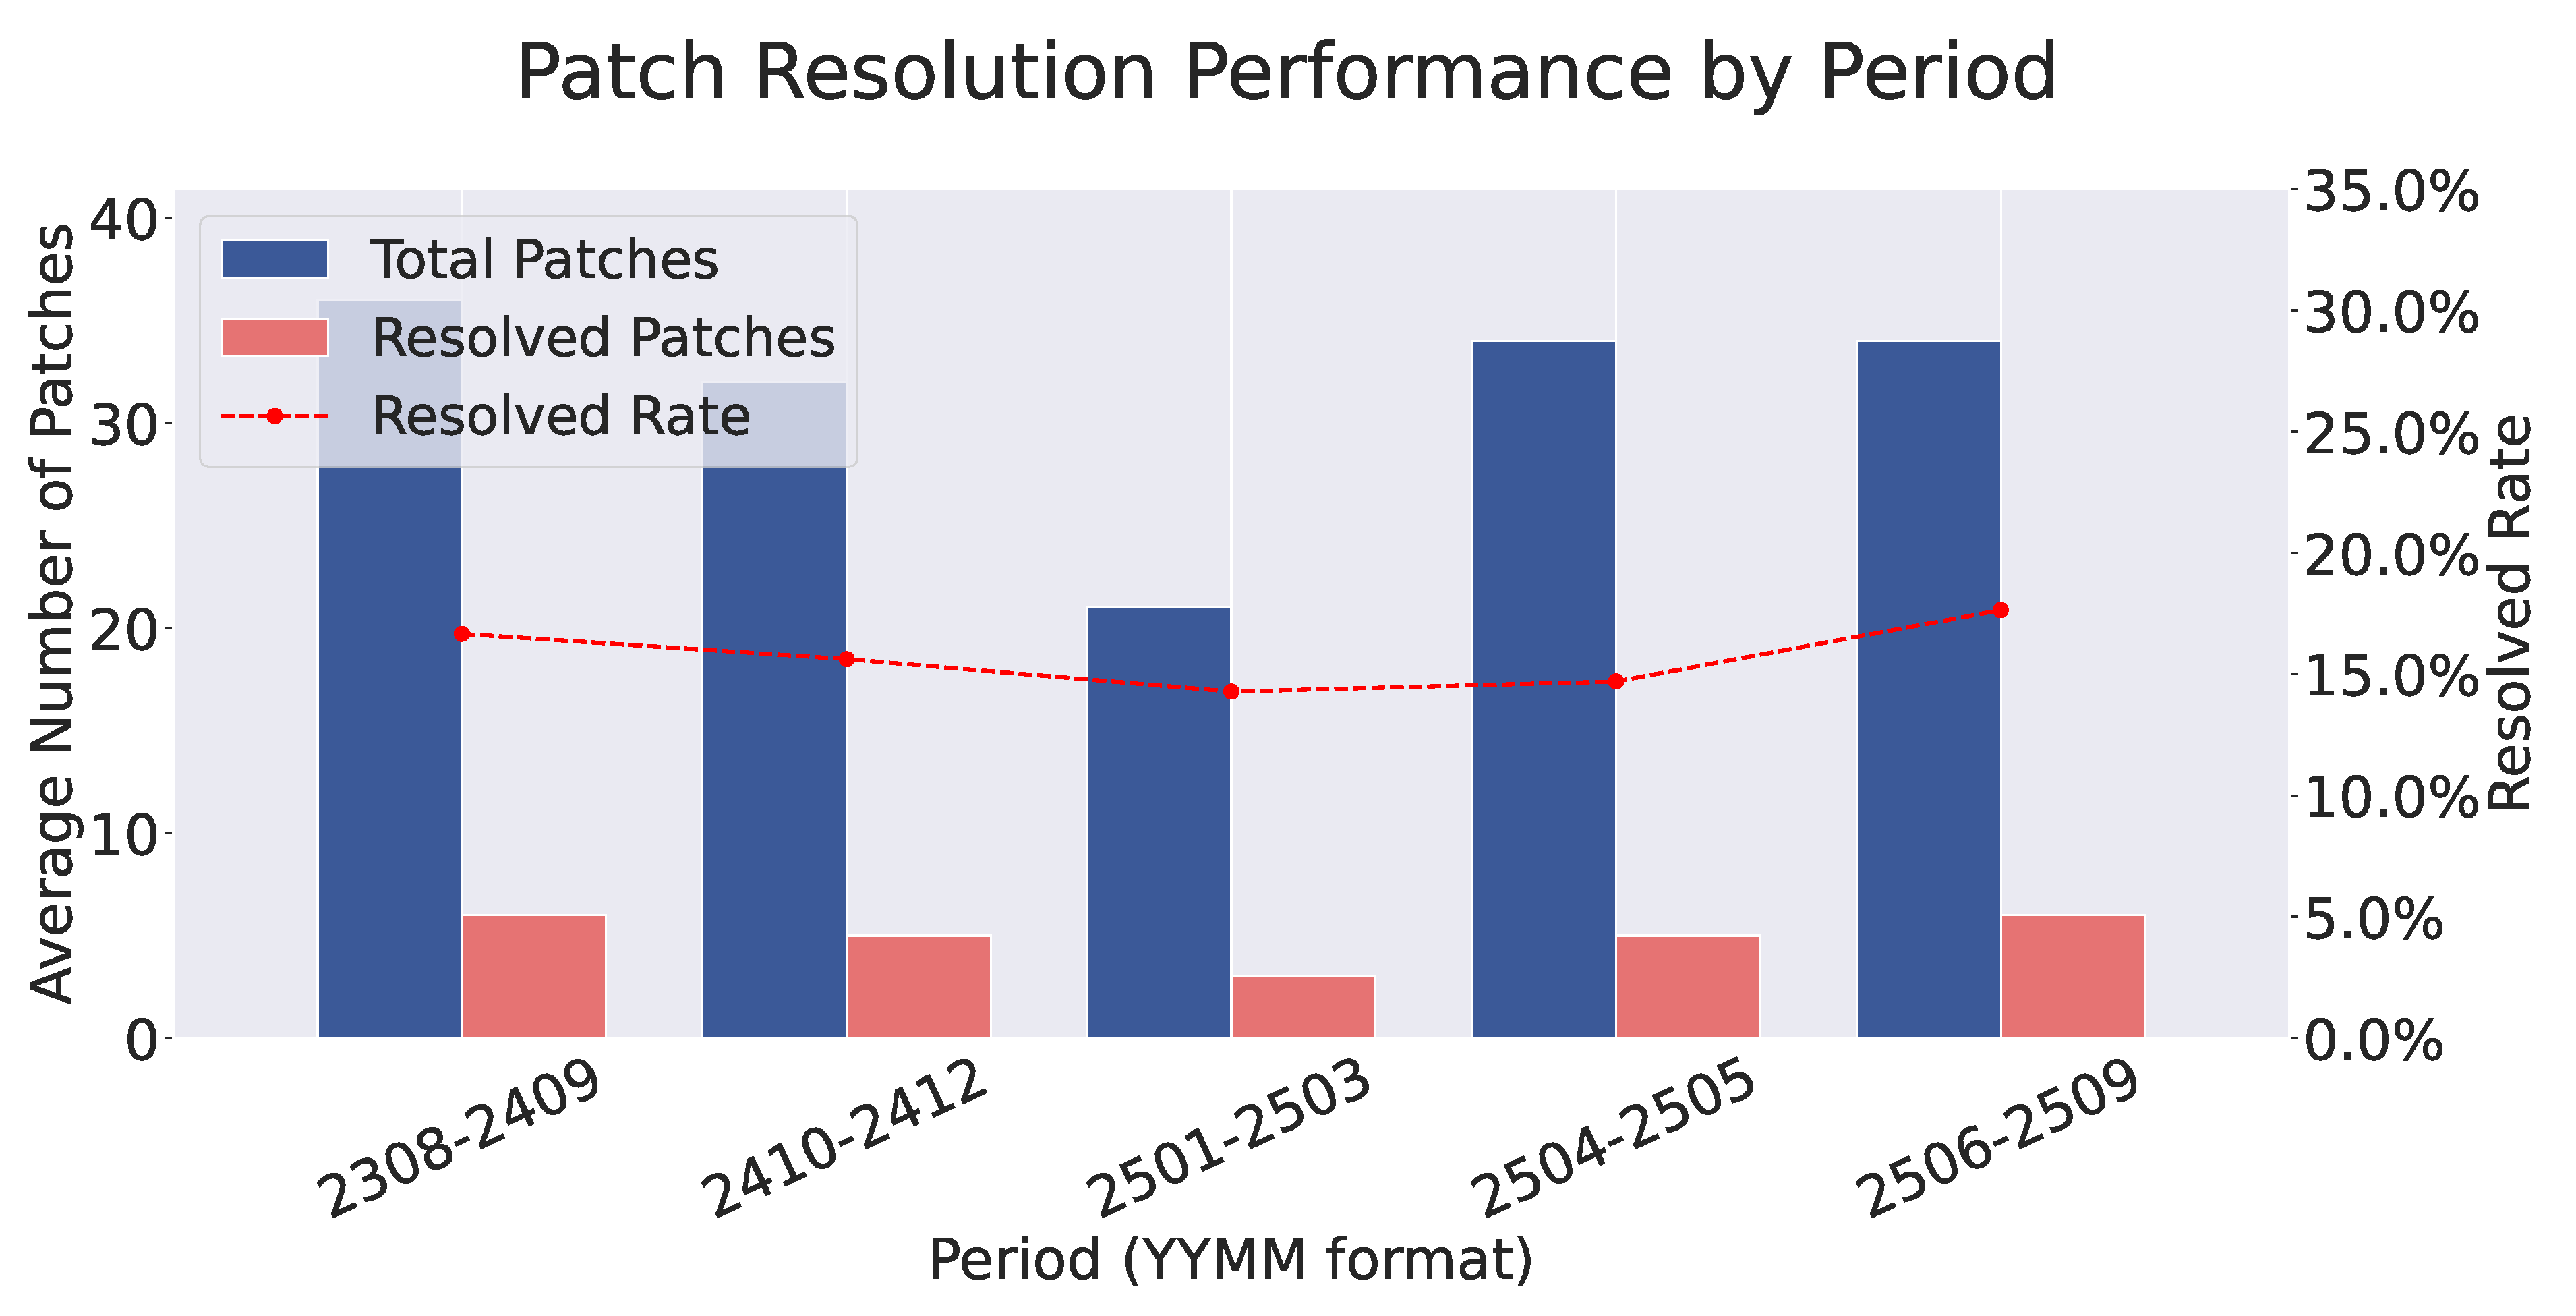
\includegraphics[width=\linewidth]{figs/Figure_3.pdf}
    \caption{Association between Resolved Rate and Creation Time.}
    \Description{A combined bar and line chart showing the stable resolved rate of approximately 20\% across five time periods.}
    \label{fig:creation_time}
    \vspace{-15pt}
\end{wrapfigure}

\paragraph{\textbf{Impact of Task Complexity.}}
The agent's success, measured by the resolved rate, is significantly influenced by complexity at both the repository and patch levels.
At the repository level, complexity is quantified by the total number of files and aggregate lines of code (LOC).
As illustrated in \cref{fig:repository_complexity}, a strong inverse correlation exists between a repository's complexity and the agent's performance.
While agents perform well on smaller repositories (fewer than 200 files or 50,000 LOC), with resolved rates reaching up to 60-70\% for GPT-5, their success degrades sharply with complexity.
In large repositories (more than 800 files or 300,000 LOC), performance for all models converges to a low of 10-30\%.
This consistent trend, which affects even top-performing models, highlights that \textbf{current LLM agents operate within a bounded scope, limiting their practical application to smaller-scale repositories rather than massive industrial systems.}

\begin{figure}[htbp]
    \centering
    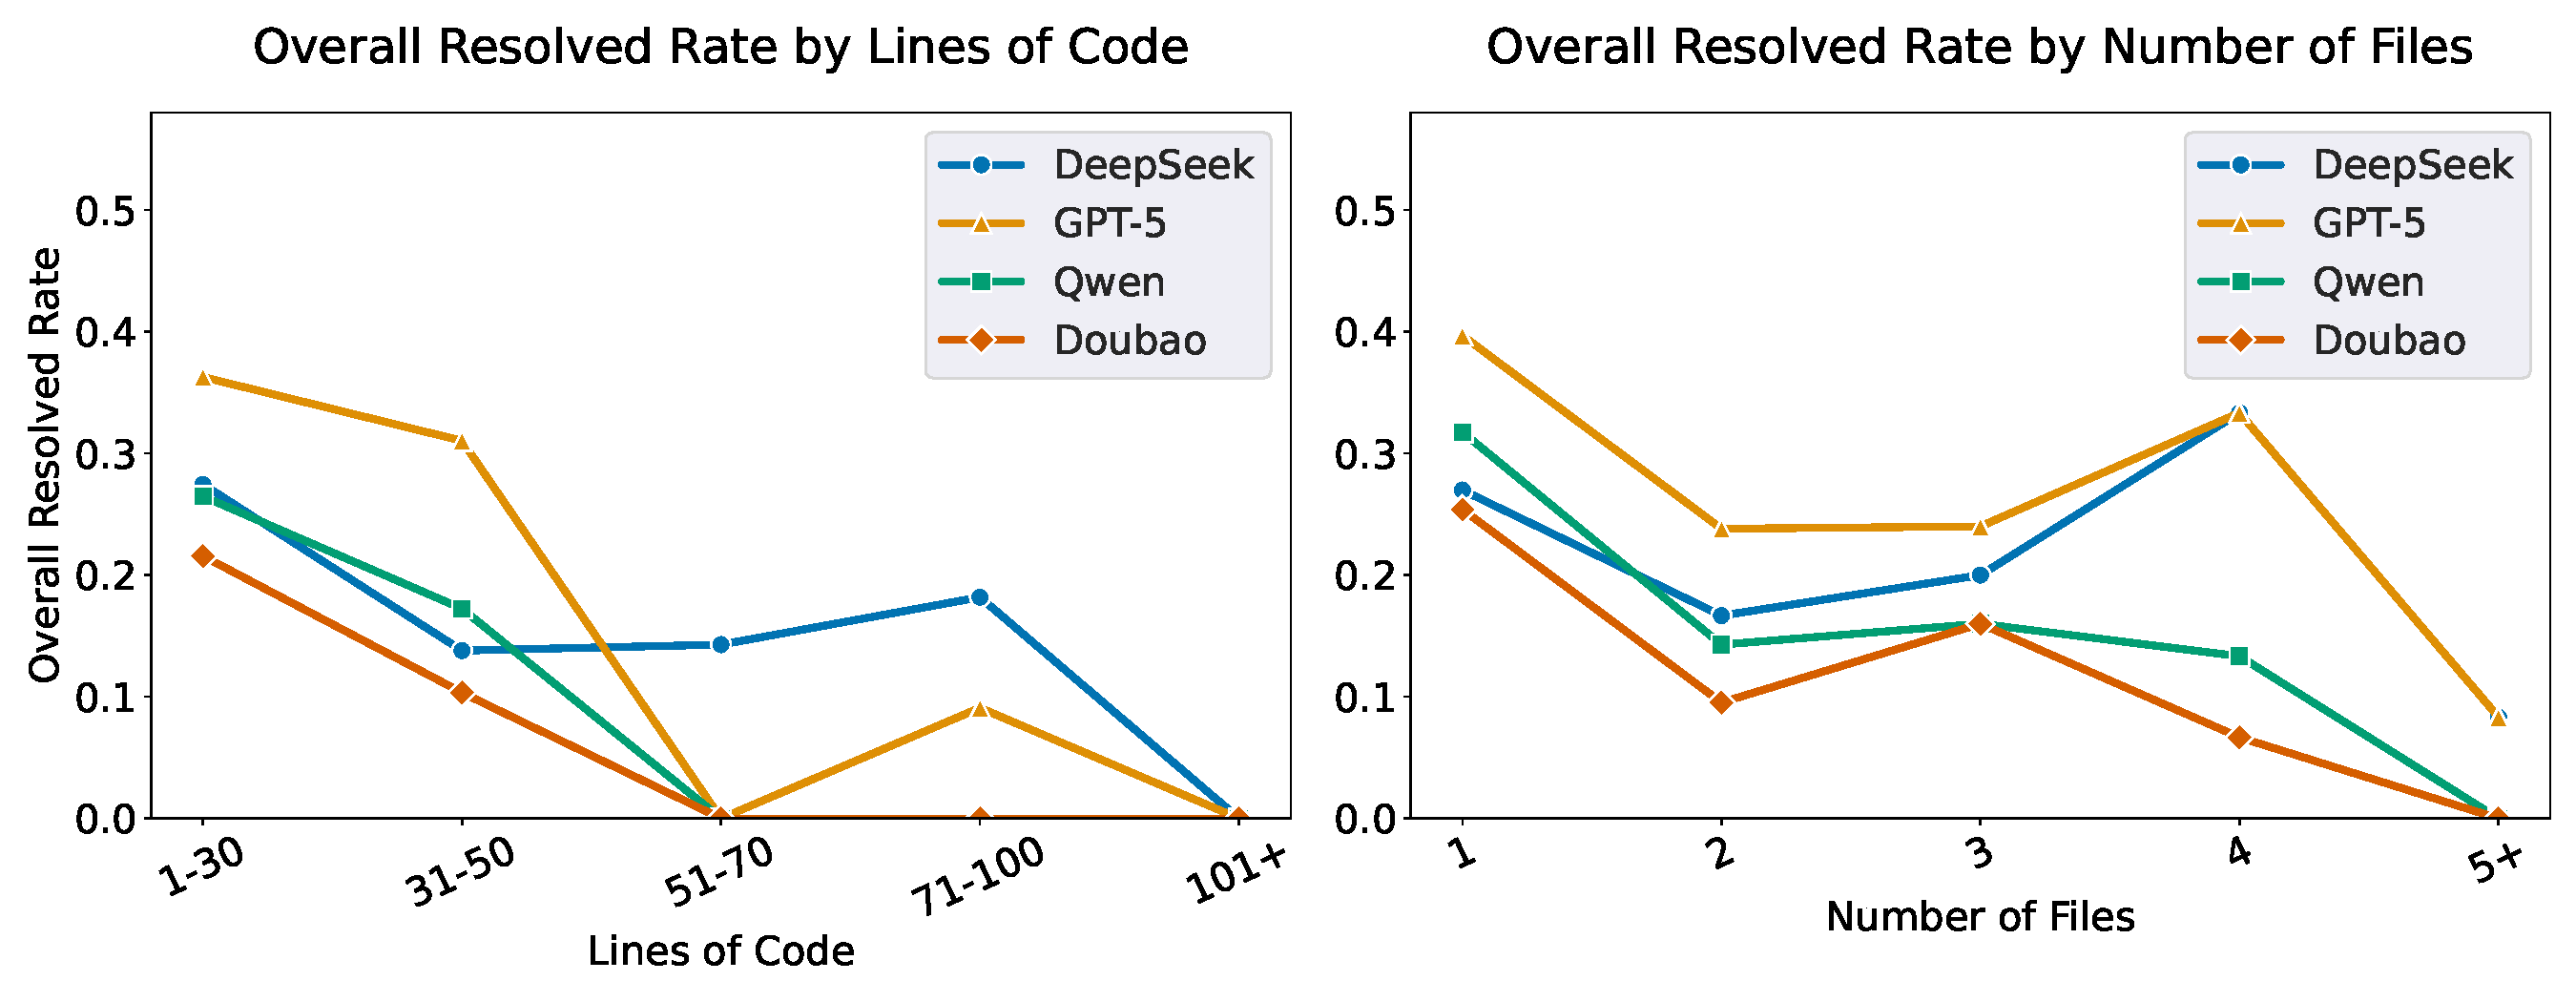
\includegraphics[width=\linewidth]{figs/Figure_2.pdf}
    \caption{Correlation Between Resolved Rate and Patch Complexity.}
    \Description{Two line charts evaluating how the complexity of the ground truth patch affects the agent's success. One chart categorizes tasks by the number of modified lines, and the other by the number of files involved. The data highlights a performance collapse for substantial modifications, particularly for patches exceeding 50 lines or spanning more than five files.}
    \label{fig:patch_complexity}
\end{figure}

Beyond the overall repository, the intrinsic complexity of the ground truth solution, or gold patch, is another critical factor.
As depicted in \cref{fig:patch_complexity}, which evaluates patch complexity based on its LOC and the number of files it spans, success rates peak for single-file patches and those between 1-30 Lines of Code (LOC), where the top model achieves a 36\% resolved rate.
However, performance collapses for substantial modifications, with success rates falling to \textbf{nearly zero} for patches exceeding 50 LOC or those distributed across five or more files.
This highlights a clear limitation in handling larger or more widespread code changes, demonstrating that \textbf{the agent's performance is highest on small, localized code changes and degrades significantly as the patch size and distribution increase.}

\paragraph{\textbf{Impact of Creation Time.}}
We further investigate the relationship between task creation time and the resolved rate to determine if model performance exhibits temporal dependency. As illustrated in \cref{fig:creation_time}, while the total volume of patches fluctuates across five distinct periods (from 2308 to 2509), the resolved rate for the Trae-agent with Doubao-Seed-1.6 remains remarkably consistent.
This stability is critical, as an upward trend in performance would suggest that data leakage from earlier tasks is being repeated in later periods.

\begin{boxK}
\textbf{RQ2 Summary:} 
We found that agent performance is strictly constrained by repository and patch complexity, limiting their practical application to smaller-scale repositories rather than massive industrial systems. Meanwhile, the consistent performance across task creation times validates the absence of data leakage.
\end{boxK}

\subsection{RQ3: Case Study}
To investigate the underlying reasons for agent failures on FeatBench, we performed a manual inspection of the failed cases. Specifically, we analyzed 122 failure cases generated by Trae-agent to identify the primary reasons for failure. This analysis was conducted by two computer science researchers from the author team, both of whom possess over two years of professional Python development experience. The identified reasons were categorized into three distinct types:
\ding{182} \textbf{Misunderstood User Requirements}, where the agent fails to bridge the gap between high-level natural language requirements and correct code implementation; \ding{183} \textbf{Incomplete Implementation}, where the agent comprehends the requirements but overlooks specific implementation details; and \ding{184} \textbf{Regressive Implementation}, where the agent successfully implements the required feature but violates reliability, breaking existing features. As shown in \cref{fig:fail_reason}, most failures fall into the third category.
This indicates that while the agent is often capable of understanding and implementing the requirements, its primary challenge lies in doing so without causing regressions that lead to test failures.

\begin{wrapfigure}{r}{0.5\linewidth}
    \centering
    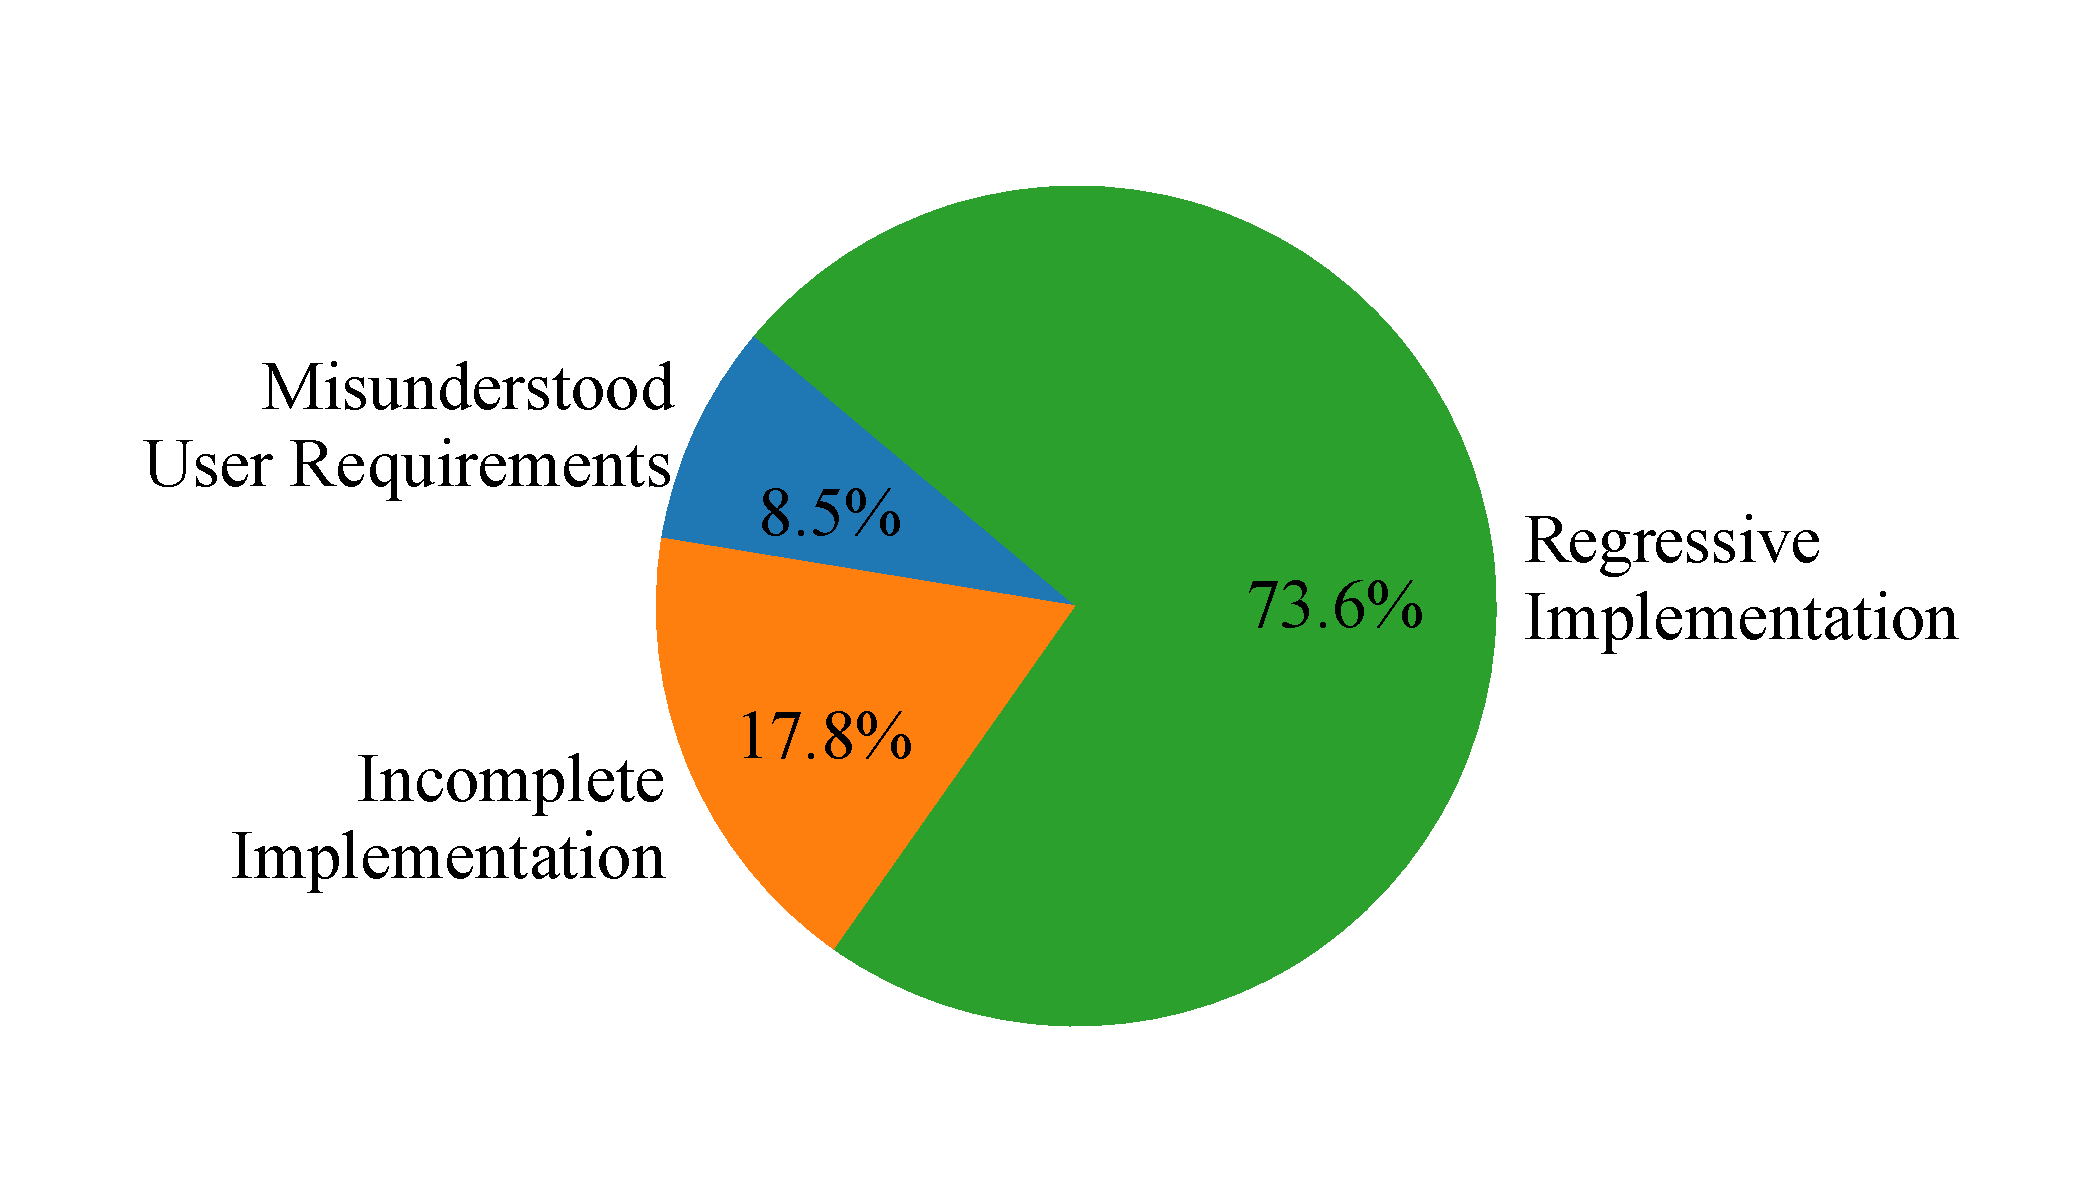
\includegraphics[width=\linewidth]{figs/Figure_7.pdf}
    \caption{Failure Reasons of Analyzed Cases.}
    \Description{A pie chart showing the distribution of failure reasons for Trae-agent: Regressive Implementation at 73.6\%, Incomplete Implementation at 17.8\%, and Misunderstood user intent at 8.5\%.}
    \label{fig:fail_reason}
\end{wrapfigure}

A clear case reveals that these regression failures are frequently driven by a behavioral pattern: Aggressive Implementation. Instead of adhering strictly to the minimal changes required to satisfy the user's requirements, agents tend to exhibit ``scope creep,'' proactively extending features or refactoring code beyond the explicit intent.
Specifically, as shown in \cref{fig:wrong}, this task's objective was to add C++26 standard support for the GCC compiler.
The gold patch correctly adhered to this scope by updating both \texttt{default\_settings.py} (to define the setting) and \texttt{flags.py} (to implement it).
In contrast, the agent-generated patch adopted the aggressive implementation, attempting to also add C++26 parameters for the Intel C++ Compiler (\texttt{intel-cc}) in \texttt{default\_settings.py}.
However, it neglected to add the corresponding implementation logic in \texttt{flags.py}. This created a configuration that was declared but not implemented, introducing a regression that caused previously passing tests reliant on \texttt{intel-cc} to fail.

\begin{figure}[t!]
    \centering
    \begin{subfigure}[t]{0.48\linewidth}
        \centering
        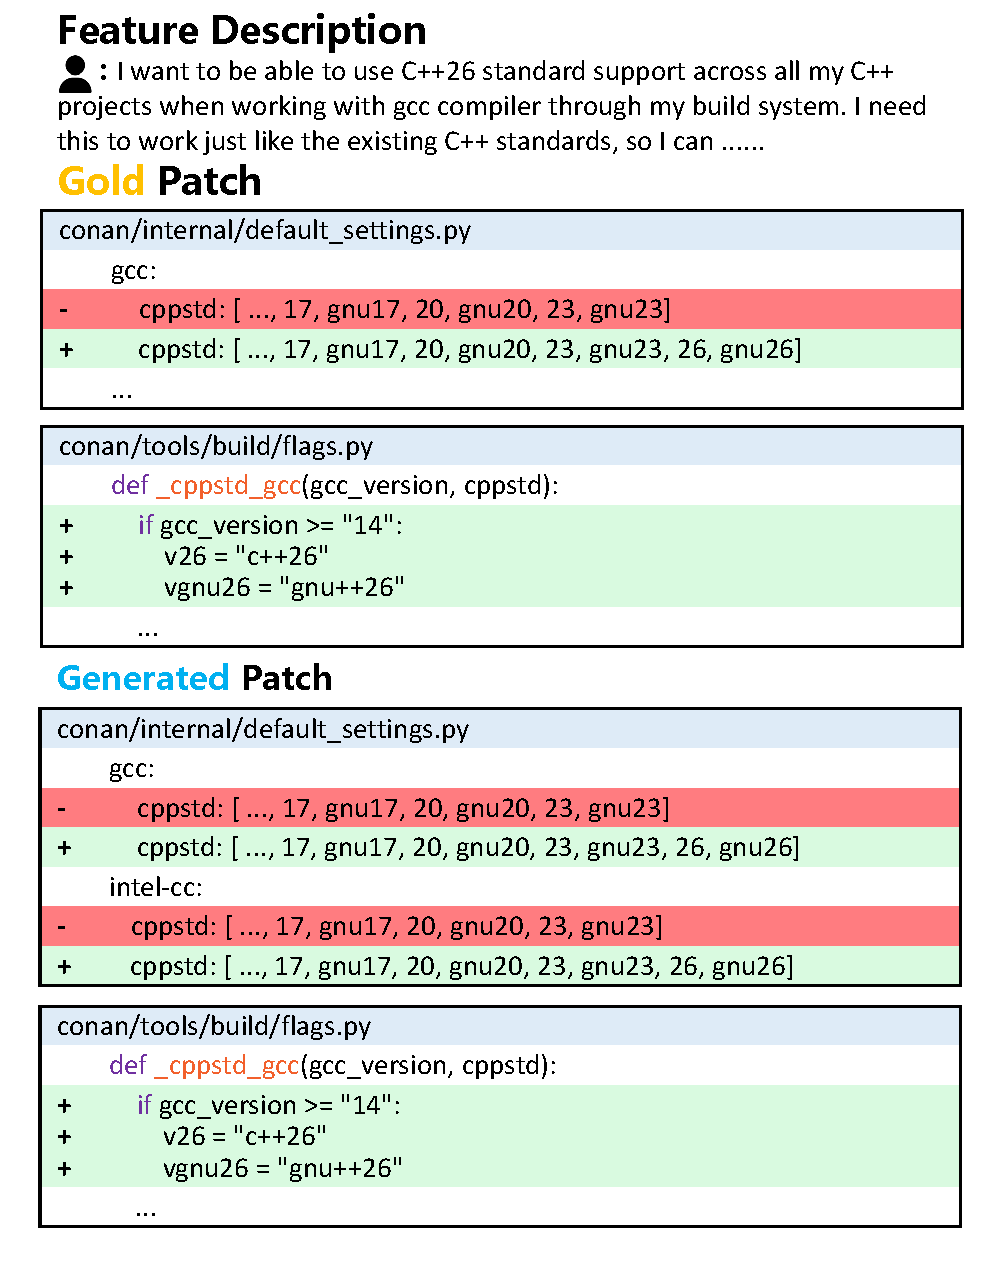
\includegraphics[width=\linewidth]{figs/fig5.pdf}
        \caption{Wrong Generated Patch from conan-io/conan\citep{conan_2025}}
        \label{fig:wrong}
    \end{subfigure}
    \hfill
    \begin{subfigure}[t]{0.48\linewidth}
        \centering
        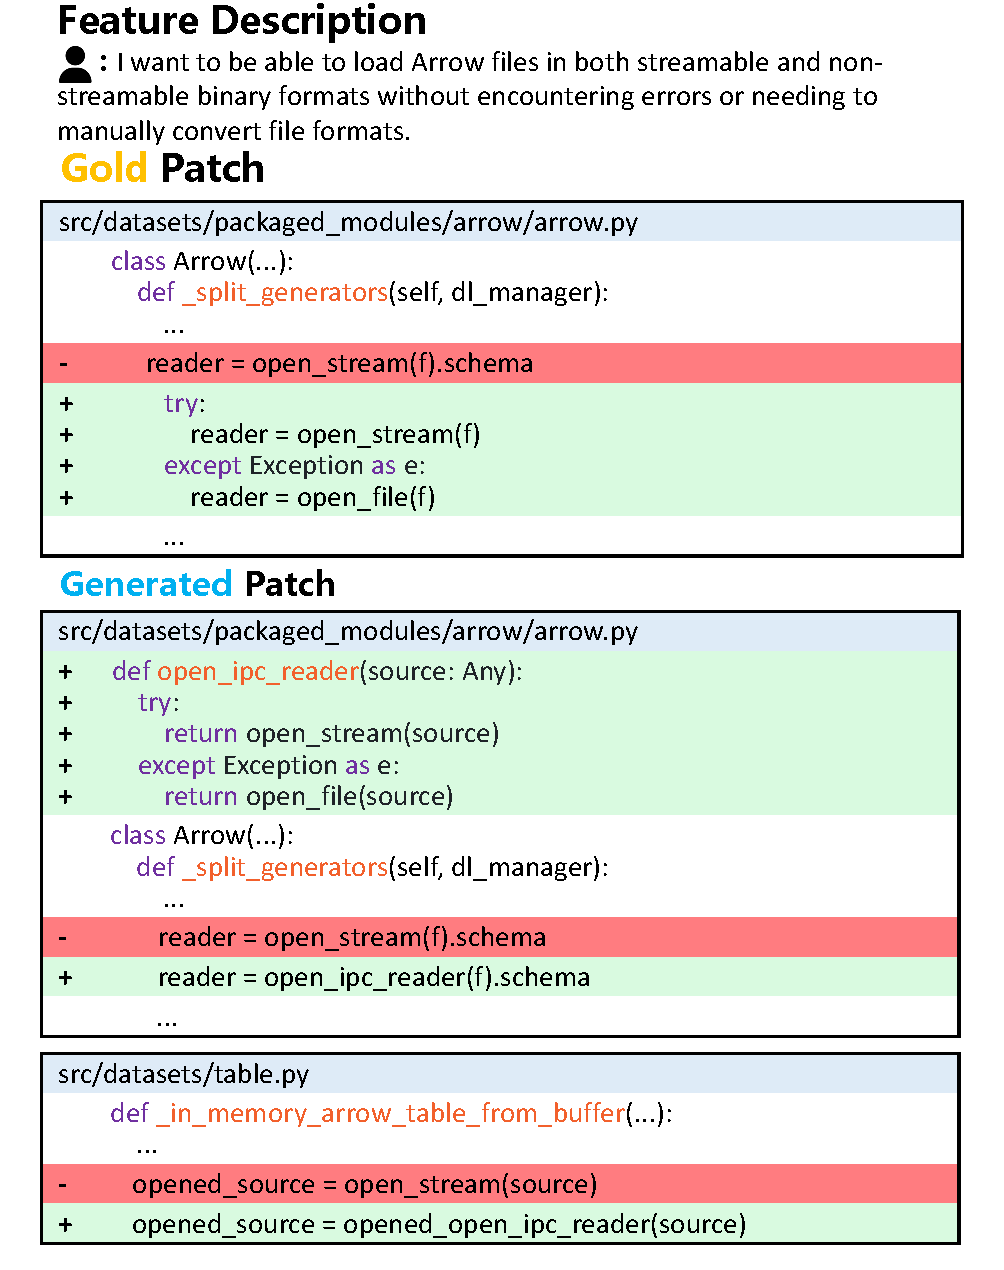
\includegraphics[width=\linewidth]{figs/fig4.pdf}
        \caption{Robust Generated Patch from huggingface/datasets\citep{huggingfacedatasets}}
        \label{fig:robust}
    \end{subfigure}
    \caption{Case Studies of Gold Patch and Generated Patch.}
    \Description{A comparative analysis of code implementation quality between an autonomous agent and a human developer. 
    Subfigure (a) illustrates an agent-generated patch from the ``conan'' repository that exhibits aggressive implementation.
    Subfigure (b) displays the human-authored gold patch from the datasets repository, demonstrating a robust architectural design that utilizes a centralized helper function for stream handling.}
    \label{fig:total}
\end{figure}

However, this behavioral pattern also yields advantages, as agent-generated code can occasionally surpass human-written patches in terms of robustness and architectural generality. For instance, \cref{fig:robust} illustrates a requirement in the \texttt{huggingface/datasets} repository to support both streamable and non-streamable Apache Arrow file loading.
The human-written gold patch, while functional, employed a localized \texttt{try-except} block in \texttt{\_split\_generators}, a non-scalable fix that would require code duplication for future extensions.
In contrast, Trae-agent implemented a more sophisticated architectural design by abstracting the core logic into a reusable helper function, \texttt{open\_ipc\_reader(source: Any)}, encapsulating the stream-opening logic and its fallbacks. By replacing direct calls with invocations of this centralized function in both \texttt{\_split\_generators} and \texttt{\_in\_memory\_arrow\_table\_from\_buffer}, the agent established a scalable pattern that improves modularity and simplifies future maintenance.

The tendency toward aggressive implementation constitutes a double-edged sword.
On one hand, as demonstrated in the failure case, an overly aggressive implementation can be detrimental, extending far beyond the original scope and introducing errors.
On the other hand, as shown in the success case, this same behavior is the mechanism behind the agent's capacity for high-level architectural optimization.
\textbf{This suggests that current SOTA agents do not merely bridge the gap between high-level user requirements and concrete code changes, but actively exceed the specified requirements to infer broader architectural needs.}
\textbf{Therefore, there is a critical need for mechanisms that can control the agent's level of aggressive implementation}, allowing this behavior to be harnessed for robust architectural improvements while preventing the harmful ``scope creep'' that introduces defects.

\begin{boxK}
\textbf{RQ3 Summary:}
The predominant cause of failure is regressive implementation, often driven by a behavioral pattern of aggressive implementation. This behavior acts as a double-edged sword: while it is the primary source of defects through unnecessary modifications, it simultaneously enables agents to generate architectural designs that are superior to human-written patches in terms of robustness and generality.
\end{boxK}